\let\negmedspace\undefined
\let\negthickspace\undefined
\documentclass[journal]{IEEEtran}
\usepackage[a5paper, margin=10mm, onecolumn]{geometry}
\usepackage{lmodern} % Ensure lmodern is loaded for pdflatex
\usepackage{tfrupee} % Include tfrupee package

\setlength{\headheight}{1cm} % Set the height of the header box
\setlength{\headsep}{0mm}     % Set the distance between the header box and the top of the text

\usepackage{gvv-book}
\usepackage{gvv}
\usepackage{cite}
\usepackage{amsmath,amssymb,amsfonts,amsthm}
\usepackage{algorithmic}
\usepackage{graphicx}
\usepackage{textcomp}
\usepackage{xcolor}
\usepackage{txfonts}
\usepackage{listings}
\usepackage{enumitem}
\usepackage{mathtools}
\usepackage{gensymb}
\usepackage{comment}
\usepackage[breaklinks=true]{hyperref}
\usepackage{tkz-euclide} 
\usepackage{listings}
\def\inputGnumericTable{}                                 
\usepackage[latin1]{inputenc}                                
\usepackage{color}                                            
\usepackage{array}                                            
\usepackage{longtable}                                       
\usepackage{calc}                                             
\usepackage{multirow}                                         
\usepackage{hhline}                                           
\usepackage{ifthen}                                           
\usepackage{lscape}

\begin{document}

\bibliographystyle{IEEEtran}
\vspace{3cm}

\title{9.ex.5}
\author{EE24BTECH11002 - Agamjot Singh}
% \maketitle
% \newpage
% \bigskip
{\let\newpage\relax\maketitle}

\renewcommand{\thefigure}{\theenumi}
\renewcommand{\thetable}{\theenumi}
\setlength{\intextsep}{10pt} % Space between text and floats

\textbf{Question:}
\newline
Solve the differential equation:
\begin{align}
  \frac{d^2y}{dx^2} + y = 0
\end{align}

\textbf{Solution:}

\textbf{Theoritical solution:} \newline
The given differential equation is a second-order linear ordinary differential equation. \newline
Let $y\brak{0} = c_1$ and $y^{\prime}\brak{0} = c_2$.
By definition of Laplace transform,
\begin{align}
    \mathcal{L}\brak{f\brak{t}} = \int_0^{\infty} e^{-st} f\brak{t} \, dt
\end{align}
Some used properties of Laplace transform include,
\begin{align}
    \mathcal{L}\brak{y^{\prime\prime}} &= s^2\mathcal{L}\brak{y} -sy\brak{0}-y^\prime\brak{0} = s^2\mathcal{L}\brak{y} -sc_1 - c_2\\
    \mathcal{L}\brak{\cos{t}} &= \frac{s}{s^2 + 1}\\
    \mathcal{L}\brak{\sin{t}} &= \frac{1}{s^2 + 1}\\
    \mathcal{L}\brak{cf\brak{t}} &= c\mathcal{L}\brak{f\brak{t}}\\
    \mathcal{L}\brak{f\brak{t}} = F\brak{s} &\implies \mathcal{L}\brak{e^{at}f\brak{t}} = F\brak{s-a}
\end{align}
Applying Laplace transform on the given differential equation, we get,
\begin{align}
    y^{\prime\prime} + y &= 0\\
    \mathcal{L}\brak{y^{\prime\prime}} + \mathcal{L}\brak{y} &= 0\\
    s^2\mathcal{L}\brak{y} - sc_1 - c_2 + \mathcal{L}\brak{y} &= 0\\
    \mathcal{L}\brak{y} &= \frac{sc_1 + c_2}{s^2 + 1} = c_1\frac{s}{s^2 + 1} + c_2\frac{1}{s^2 + 1} \label{laplace_eq}\\
\end{align}
Taking laplace inverse on both sides, we get,
\begin{align}
    y &= c_1\mathcal{L}^{-1}\brak{\frac{s}{s^2 + 1}} + c_2\mathcal{L}^{-1}\brak{\frac{1}{s^2 + 1}}\\
    y &= c_1\cos{x} + c_2\sin{x}\\
    \implies y\brak{x} &= \sqrt{\brak{c_1}^2 + \brak{c_2}^2} \sin{\brak{x + \tan^{-1}{\brak{\frac{c_1}{c_2}}}}}
\end{align}

\textbf{Computational Solution:} Trapezoid Method
\newline
The given differential equation can be represented as 
\begin{align}
    y^{\prime\prime} + y = 0
\end{align}
Let $y = y_1$ and $y^{\prime} = y_2$, then, 
\begin{align}
    \frac{dy_2}{dx} &= -y_1 \text{ and } \frac{dy_1}{dx} = y_2\\
    \int_{y_{2, n}}^{y_{2, n + 1}} \, dy_2 &= \int_{x_n}^{x_{n + 1}} -y_1 \, dx\\
    \int_{y_{1, n}}^{y_{1, n + 1}} \, dy_1 &= \int_{x_n}^{x_{n + 1}} y_2 \, dx\\
\end{align}
Discretizing the steps \brak{\text{Trapezoid rule}},
\begin{align}
    y_{2, n + 1} - y_{2, n} &= -\frac{h}{2}\brak{y_{1, n} + y_{1, n + 1}}\\
    y_{1, n + 1} - y_{1, n} &= \frac{h}{2}\brak{y_{2, n} + y_{2, n + 1}}
\end{align}
Solving for $y_{1, n + 1}$ and $y_{2, n + 1}$, we get,
\begin{align}
    y_{1, n + 1} = y_{1, n} + \frac{h}{2}\brak{2y_{2, n} - \frac{h}{2}\brak{y_{1, n} + y_{1, n + 1}}}\\
\end{align}
The difference equations can be written as,
\begin{align}
    y_{1, n + 1} = \frac{\brak{4 - h^2}y_{1, n} + 4hy_{2, n}}{\brak{4 + h^2}}\\
    y_{2, n + 1} = \frac{\brak{4 - h^2}y_{2, n} - 4hy_{1, n}}{\brak{4 + h^2}}\\
\end{align}

Iteratively plotting the above system taking intial conditions as 
\begin{align}
    x_0 = 0 \text{ , } y_{1, 0} = 0 \text{ , } y_{2, 0} = 1
\end{align}
we get the plot of the given differential equation.

\textbf{Alternative Computational Solution:} Bilinear transform 
\newline
We have to apply laplace transformation on the given differential equation. From \brak{\ref{laplace_eq}}, we get,
\begin{align}
    Y\brak{s} &= \frac{sc_1 + c_2}{s^2 + 1}
\end{align}
\begin{align}
    Y\brak{s} &= \frac{sc_1 + c_2}{s^2 + 1}
\end{align}
Applying Bilinear transform, with $T = h$, we get,
\begin{align}
    s &= \frac{2}{T}\frac{1 - z^{-1}}{1 + z^{-1}} = \frac{2}{h}\frac{1 - z^{-1}}{1 + z^{-1}}\\
    \implies Y\brak{z} &= \frac{2hc_1 \brak{z^2 - 1} + c_2h^2 \brak{z + 1}^2}{\brak{h^2 + 4}z^2 + 2\brak{h^2 - 4}z + \brak{h^2 + 4}}\\
    \implies \brak{z^2 + 2\frac{h^2 - 4}{h^2 + 4}z + 1} Y\brak{z} &= 2hc_1 \brak{z^2 - 1} + c_2h^2 \brak{z^2 + 2z + 1}\\
    \implies z^2Y\brak{z} + 2\frac{h^2 - 4}{h^2 + 4}zY\brak{z} + Y\brak{z} &= \brak{2h c_1 + c_2 h^2}z^2 + \brak{2h^2 c_2}z + \brak{h^2c_2 - 2hc_1} \label{bilinear_eq}
\end{align}
Some properties of one sided $z$ transform,
\begin{align}
    \mathcal{Z}\brak{y\sbrak{n + 2}} &= z^2 Y\brak{z} - y\sbrak{1}z - y\sbrak{0}\\
    \mathcal{Z}\brak{y\sbrak{n + 1}} &= z Y\brak{z} - z y_\sbrak{0}\\
    \mathcal{Z}\brak{\delta\sbrak{n}} &= 1 \text{, } z \neq 0\\
    \mathcal{Z}\brak{y\sbrak{n}} = Y\brak{z} &\implies \mathcal{Z}\brak{y\sbrak{n - n_0}} = z^{-n_0}Y\brak{z} \label{time_shift_eq}
\end{align}
By the time shift property $\brak{\ref{time_shift_eq}}$,
\begin{align}
    \mathcal{Z}\brak{\delta\sbrak{n + 2}} &= z^2 \text{, } z \neq 0\\
    \mathcal{Z}\brak{\delta\sbrak{n + 1}} &= z \text{, } z \neq 0
\end{align}
Rewriting equation $\brak{\ref{bilinear_eq}}$, we get,
\begin{align}
    \implies z^2Y\brak{z} + 2\frac{h^2 - 4}{h^2 + 4}zY\brak{z} + Y\brak{z} &= \brak{2h c_1 + c_2 h^2}z^2 + \brak{2h^2 c_2}z + \brak{h^2c_2 - 2hc_1}
\end{align}
Taking $z$ inverse transform on both sides of equation $\brak{\ref{bilinear_eq}}$,
\begin{align}
    hello
\end{align}

\begin{figure}[h!]
    \centering
    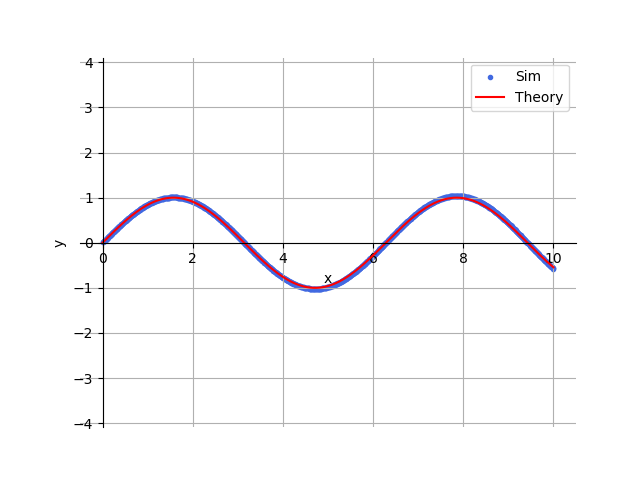
\includegraphics[width=0.7\columnwidth]{figs/graph.png}
    \caption{Computational solution for $y^{\prime\prime} + y = 0$}
    \label{label}
\end{figure}

\end{document}
